\documentclass[twoside]{book}

% Packages required by doxygen
\usepackage{fixltx2e}
\usepackage{calc}
\usepackage{doxygen}
\usepackage[export]{adjustbox} % also loads graphicx
\usepackage{graphicx}
\usepackage[utf8]{inputenc}
\usepackage{makeidx}
\usepackage{multicol}
\usepackage{multirow}
\PassOptionsToPackage{warn}{textcomp}
\usepackage{textcomp}
\usepackage[nointegrals]{wasysym}
\usepackage[table]{xcolor}

% Font selection
\usepackage[T1]{fontenc}
\usepackage[scaled=.90]{helvet}
\usepackage{courier}
\usepackage{amssymb}
\usepackage{sectsty}
\renewcommand{\familydefault}{\sfdefault}
\allsectionsfont{%
  \fontseries{bc}\selectfont%
  \color{darkgray}%
}
\renewcommand{\DoxyLabelFont}{%
  \fontseries{bc}\selectfont%
  \color{darkgray}%
}
\newcommand{\+}{\discretionary{\mbox{\scriptsize$\hookleftarrow$}}{}{}}

% Page & text layout
\usepackage{geometry}
\geometry{%
  a4paper,%
  top=2.5cm,%
  bottom=2.5cm,%
  left=2.5cm,%
  right=2.5cm%
}
\tolerance=750
\hfuzz=15pt
\hbadness=750
\setlength{\emergencystretch}{15pt}
\setlength{\parindent}{0cm}
\setlength{\parskip}{3ex plus 2ex minus 2ex}
\makeatletter
\renewcommand{\paragraph}{%
  \@startsection{paragraph}{4}{0ex}{-1.0ex}{1.0ex}{%
    \normalfont\normalsize\bfseries\SS@parafont%
  }%
}
\renewcommand{\subparagraph}{%
  \@startsection{subparagraph}{5}{0ex}{-1.0ex}{1.0ex}{%
    \normalfont\normalsize\bfseries\SS@subparafont%
  }%
}
\makeatother

% Headers & footers
\usepackage{fancyhdr}
\pagestyle{fancyplain}
\fancyhead[LE]{\fancyplain{}{\bfseries\thepage}}
\fancyhead[CE]{\fancyplain{}{}}
\fancyhead[RE]{\fancyplain{}{\bfseries\leftmark}}
\fancyhead[LO]{\fancyplain{}{\bfseries\rightmark}}
\fancyhead[CO]{\fancyplain{}{}}
\fancyhead[RO]{\fancyplain{}{\bfseries\thepage}}
\fancyfoot[LE]{\fancyplain{}{}}
\fancyfoot[CE]{\fancyplain{}{}}
\fancyfoot[RE]{\fancyplain{}{\bfseries\scriptsize Generated by Doxygen }}
\fancyfoot[LO]{\fancyplain{}{\bfseries\scriptsize Generated by Doxygen }}
\fancyfoot[CO]{\fancyplain{}{}}
\fancyfoot[RO]{\fancyplain{}{}}
\renewcommand{\footrulewidth}{0.4pt}
\renewcommand{\chaptermark}[1]{%
  \markboth{#1}{}%
}
\renewcommand{\sectionmark}[1]{%
  \markright{\thesection\ #1}%
}

% Indices & bibliography
\usepackage{natbib}
\usepackage[titles]{tocloft}
\setcounter{tocdepth}{3}
\setcounter{secnumdepth}{5}
\makeindex

% Hyperlinks (required, but should be loaded last)
\usepackage{ifpdf}
\ifpdf
  \usepackage[pdftex,pagebackref=true]{hyperref}
\else
  \usepackage[ps2pdf,pagebackref=true]{hyperref}
\fi
\hypersetup{%
  colorlinks=true,%
  linkcolor=blue,%
  citecolor=blue,%
  unicode%
}

% Custom commands
\newcommand{\clearemptydoublepage}{%
  \newpage{\pagestyle{empty}\cleardoublepage}%
}

\usepackage{caption}
\captionsetup{labelsep=space,justification=centering,font={bf},singlelinecheck=off,skip=4pt,position=top}

%===== C O N T E N T S =====

\begin{document}

% Titlepage & ToC
\hypersetup{pageanchor=false,
             bookmarksnumbered=true,
             pdfencoding=unicode
            }
\pagenumbering{roman}
\begin{titlepage}
\vspace*{7cm}
\begin{center}%
{\Large 3d final }\\
\vspace*{1cm}
{\large Generated by Doxygen 1.8.11}\\
\end{center}
\end{titlepage}
\clearemptydoublepage
\tableofcontents
\clearemptydoublepage
\pagenumbering{arabic}
\hypersetup{pageanchor=true}

%--- Begin generated contents ---
\chapter{Hierarchical Index}
\section{Class Hierarchy}
This inheritance list is sorted roughly, but not completely, alphabetically\+:\begin{DoxyCompactList}
\item Mono\+Behaviour\begin{DoxyCompactList}
\item \contentsline{section}{Audio\+Play}{\pageref{class_audio_play}}{}
\item \contentsline{section}{bomb\+Movement}{\pageref{classbomb_movement}}{}
\item \contentsline{section}{camera\+Control}{\pageref{classcamera_control}}{}
\item \contentsline{section}{choosechar}{\pageref{classchoosechar}}{}
\item \contentsline{section}{Dimond\+Movement}{\pageref{class_dimond_movement}}{}
\item \contentsline{section}{game\+System}{\pageref{classgame_system}}{}
\item \contentsline{section}{item\+Generator}{\pageref{classitem_generator}}{}
\item \contentsline{section}{menu}{\pageref{classmenu}}{}
\item \contentsline{section}{Player\+Health}{\pageref{class_player_health}}{}
\item \contentsline{section}{tornado\+Movement}{\pageref{classtornado_movement}}{}
\end{DoxyCompactList}
\item State\+Machine\+Behaviour\begin{DoxyCompactList}
\item \contentsline{section}{sound}{\pageref{classsound}}{}
\end{DoxyCompactList}
\end{DoxyCompactList}

\chapter{Class Index}
\section{Class List}
Here are the classes, structs, unions and interfaces with brief descriptions\+:\begin{DoxyCompactList}
\item\contentsline{section}{\hyperlink{class_audio_play}{Audio\+Play} }{\pageref{class_audio_play}}{}
\item\contentsline{section}{\hyperlink{classbomb_movement}{bomb\+Movement} }{\pageref{classbomb_movement}}{}
\item\contentsline{section}{\hyperlink{classcamera_control}{camera\+Control} }{\pageref{classcamera_control}}{}
\item\contentsline{section}{\hyperlink{classchoosechar}{choosechar} }{\pageref{classchoosechar}}{}
\item\contentsline{section}{\hyperlink{class_dimond_movement}{Dimond\+Movement} }{\pageref{class_dimond_movement}}{}
\item\contentsline{section}{\hyperlink{classgame_system}{game\+System} }{\pageref{classgame_system}}{}
\item\contentsline{section}{\hyperlink{classitem_generator}{item\+Generator} }{\pageref{classitem_generator}}{}
\item\contentsline{section}{\hyperlink{classmenu}{menu} }{\pageref{classmenu}}{}
\item\contentsline{section}{\hyperlink{class_player_health}{Player\+Health} }{\pageref{class_player_health}}{}
\item\contentsline{section}{\hyperlink{classsound}{sound} }{\pageref{classsound}}{}
\item\contentsline{section}{\hyperlink{classtornado_movement}{tornado\+Movement} }{\pageref{classtornado_movement}}{}
\end{DoxyCompactList}

\chapter{Class Documentation}
\hypertarget{class_audio_play}{}\section{Audio\+Play Class Reference}
\label{class_audio_play}\index{Audio\+Play@{Audio\+Play}}
Inheritance diagram for Audio\+Play\+:\begin{figure}[H]
\begin{center}
\leavevmode
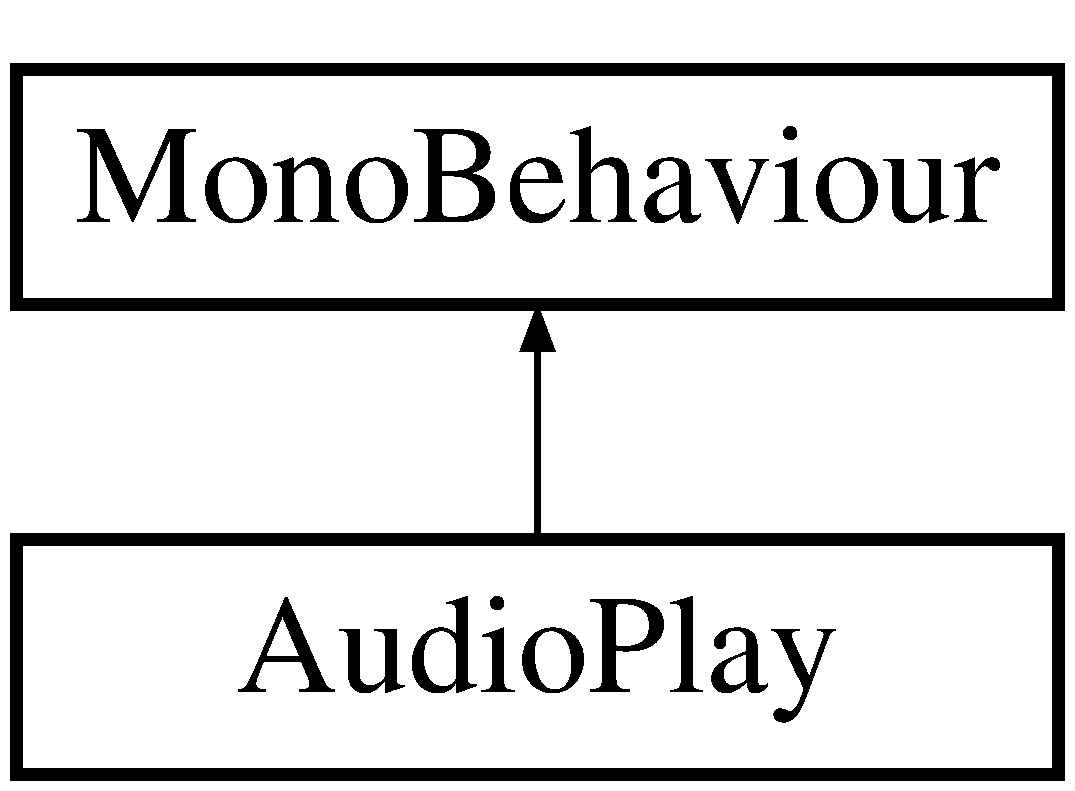
\includegraphics[height=2.000000cm]{class_audio_play}
\end{center}
\end{figure}
\subsection*{Static Public Member Functions}
\begin{DoxyCompactItemize}
\item 
static void {\bfseries play\+Sound} (Audio\+Clip clip, Audio\+Source audio\+Player)\hypertarget{class_audio_play_a0b0d431f02a57ceda1883b6687b08c95}{}\label{class_audio_play_a0b0d431f02a57ceda1883b6687b08c95}

\end{DoxyCompactItemize}


The documentation for this class was generated from the following file\+:\begin{DoxyCompactItemize}
\item 
Assets/\+Scripts/Audio\+Play.\+cs\end{DoxyCompactItemize}

\hypertarget{classbomb_movement}{}\section{bomb\+Movement Class Reference}
\label{classbomb_movement}\index{bomb\+Movement@{bomb\+Movement}}
Inheritance diagram for bomb\+Movement\+:\begin{figure}[H]
\begin{center}
\leavevmode
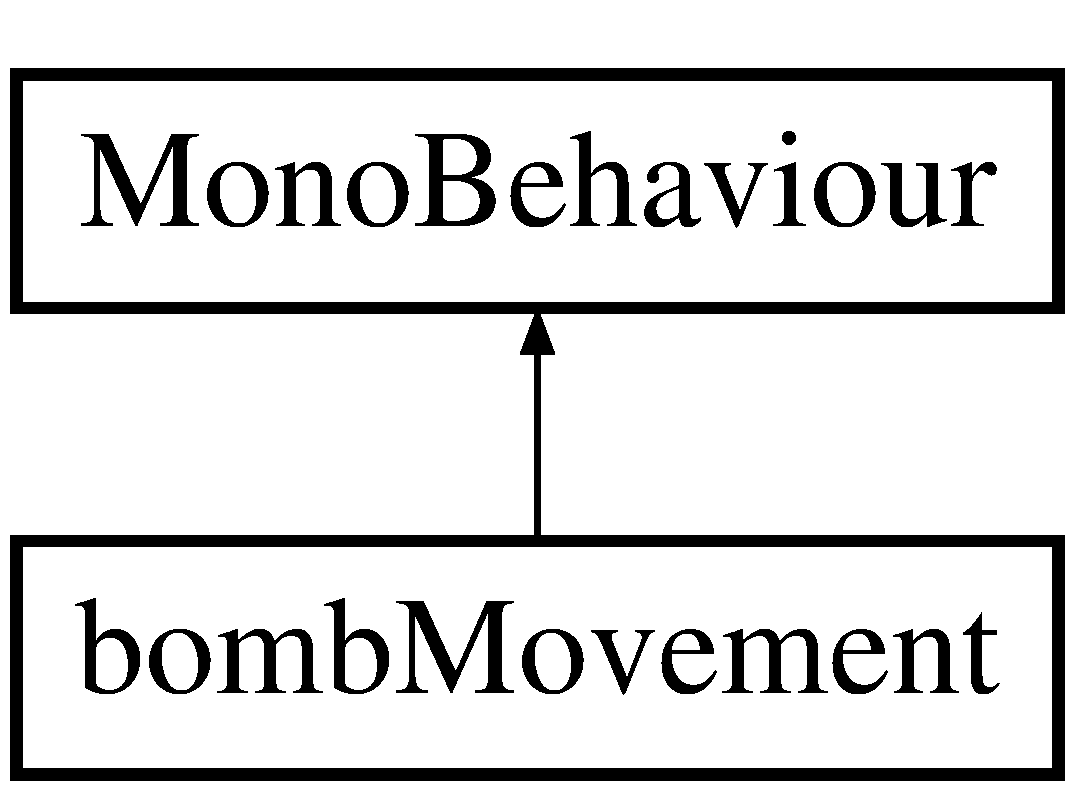
\includegraphics[height=2.000000cm]{classbomb_movement}
\end{center}
\end{figure}


The documentation for this class was generated from the following file\+:\begin{DoxyCompactItemize}
\item 
Assets/\+Scripts/bomb\+Movement.\+cs\end{DoxyCompactItemize}

\hypertarget{classcamera_control}{}\section{camera\+Control Class Reference}
\label{classcamera_control}\index{camera\+Control@{camera\+Control}}
Inheritance diagram for camera\+Control\+:\begin{figure}[H]
\begin{center}
\leavevmode
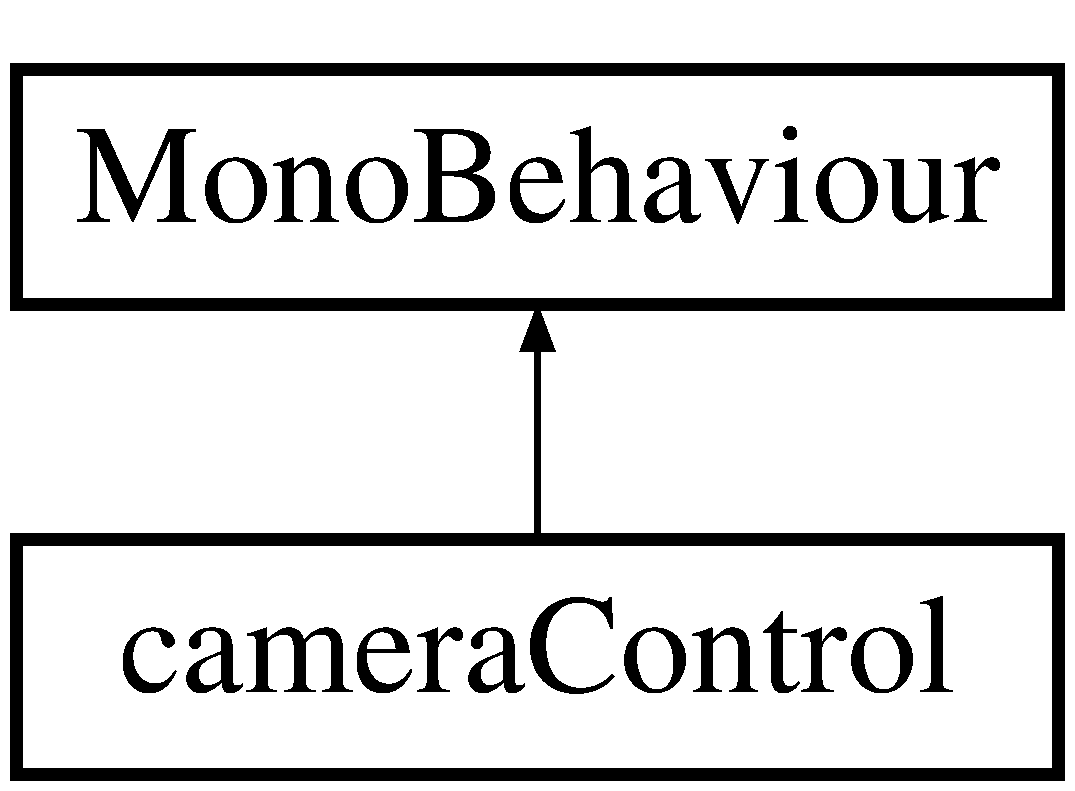
\includegraphics[height=2.000000cm]{classcamera_control}
\end{center}
\end{figure}
\subsection*{Public Attributes}
\begin{DoxyCompactItemize}
\item 
Game\+Object {\bfseries player1}\hypertarget{classcamera_control_a0f0e859e0dd7a8e8b01684027339844f}{}\label{classcamera_control_a0f0e859e0dd7a8e8b01684027339844f}

\item 
Game\+Object {\bfseries player2}\hypertarget{classcamera_control_a611122e2cbfe588d75fec370adbab75f}{}\label{classcamera_control_a611122e2cbfe588d75fec370adbab75f}

\item 
bool {\bfseries camera\+Control\+Enable} =true\hypertarget{classcamera_control_ac77ad072b488e86a1ef004297ae7e117}{}\label{classcamera_control_ac77ad072b488e86a1ef004297ae7e117}

\end{DoxyCompactItemize}


The documentation for this class was generated from the following file\+:\begin{DoxyCompactItemize}
\item 
Assets/\+Scripts/camera\+Control.\+cs\end{DoxyCompactItemize}

\hypertarget{classchoosechar}{}\section{choosechar Class Reference}
\label{classchoosechar}\index{choosechar@{choosechar}}
Inheritance diagram for choosechar\+:\begin{figure}[H]
\begin{center}
\leavevmode
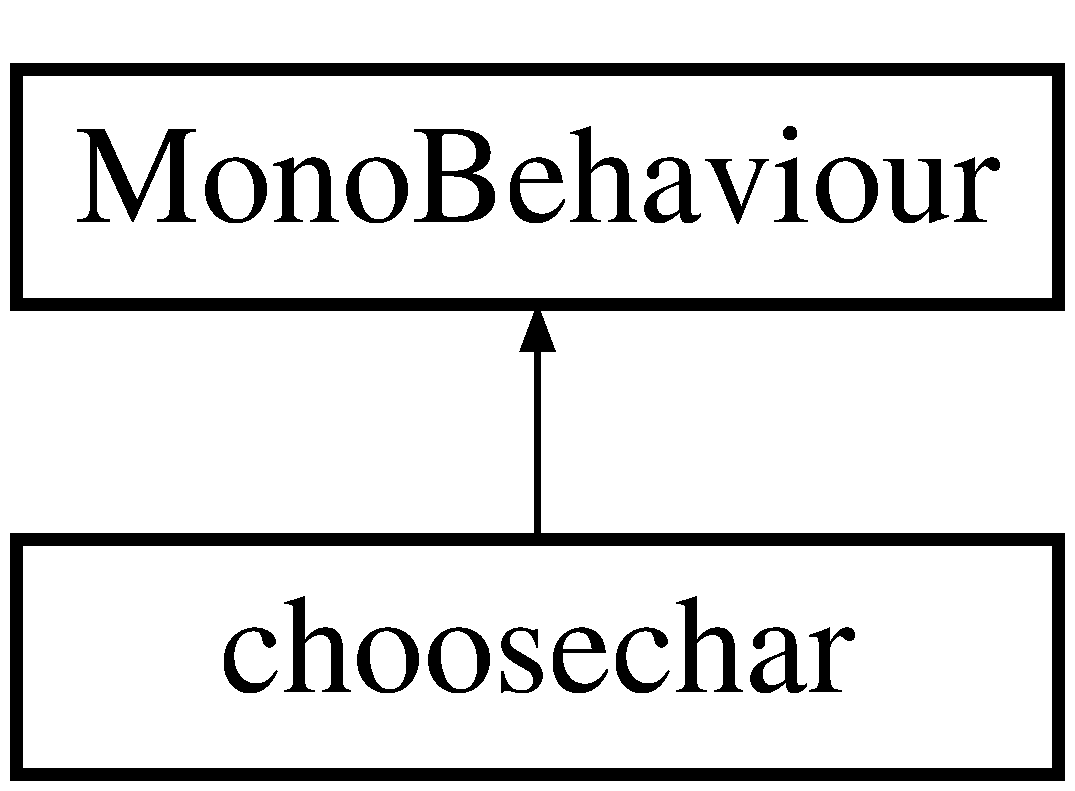
\includegraphics[height=2.000000cm]{classchoosechar}
\end{center}
\end{figure}


The documentation for this class was generated from the following file\+:\begin{DoxyCompactItemize}
\item 
Assets/\+Scripts/choosechar.\+cs\end{DoxyCompactItemize}

\hypertarget{class_dimond_movement}{}\section{Dimond\+Movement Class Reference}
\label{class_dimond_movement}\index{Dimond\+Movement@{Dimond\+Movement}}
Inheritance diagram for Dimond\+Movement\+:\begin{figure}[H]
\begin{center}
\leavevmode
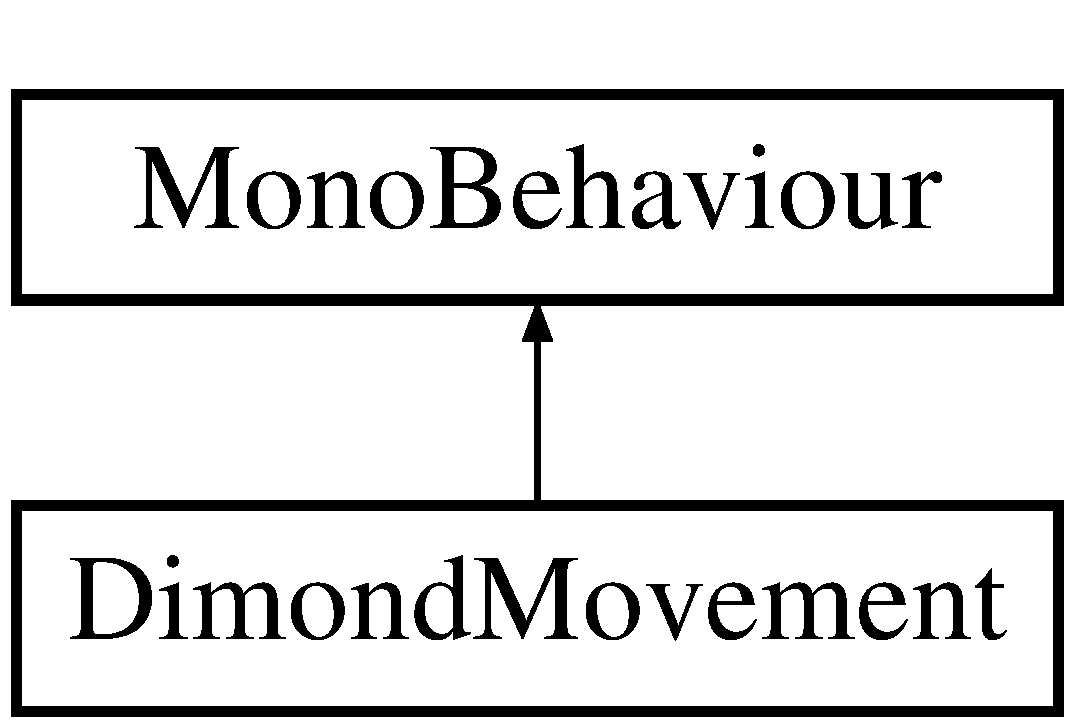
\includegraphics[height=2.000000cm]{class_dimond_movement}
\end{center}
\end{figure}


The documentation for this class was generated from the following file\+:\begin{DoxyCompactItemize}
\item 
Assets/\+Scripts/Dimond\+Movement.\+cs\end{DoxyCompactItemize}

\hypertarget{classgame_system}{}\section{game\+System Class Reference}
\label{classgame_system}\index{game\+System@{game\+System}}
Inheritance diagram for game\+System\+:\begin{figure}[H]
\begin{center}
\leavevmode
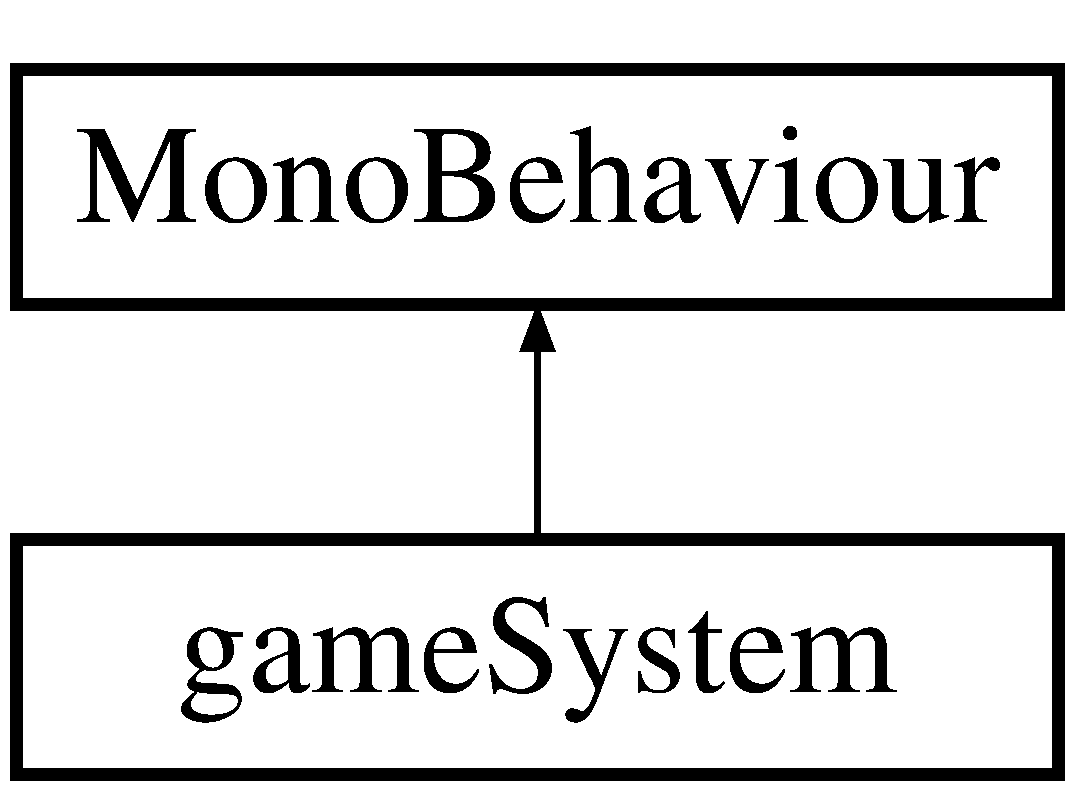
\includegraphics[height=2.000000cm]{classgame_system}
\end{center}
\end{figure}
\subsection*{Public Member Functions}
\begin{DoxyCompactItemize}
\item 
void {\bfseries set\+Winner} (int win)\hypertarget{classgame_system_a1a4828b46a992e71baf24612cd3ee589}{}\label{classgame_system_a1a4828b46a992e71baf24612cd3ee589}

\end{DoxyCompactItemize}
\subsection*{Static Public Member Functions}
\begin{DoxyCompactItemize}
\item 
static Game\+Object\mbox{[}$\,$\mbox{]} {\bfseries Find\+Game\+Objects\+With\+Tag} (string tag)\hypertarget{classgame_system_aaa3783c37d97151c299f7c4280729f43}{}\label{classgame_system_aaa3783c37d97151c299f7c4280729f43}

\item 
static Game\+Object {\bfseries Find\+With\+Tag} (string tag)\hypertarget{classgame_system_a2cd294b644b6e244cee6eb151a25e4bc}{}\label{classgame_system_a2cd294b644b6e244cee6eb151a25e4bc}

\end{DoxyCompactItemize}
\subsection*{Public Attributes}
\begin{DoxyCompactItemize}
\item 
Game\+Object {\bfseries game\+Begin\+Text}\hypertarget{classgame_system_a6c6ed1bd09eeba15452b9ac4a40321ba}{}\label{classgame_system_a6c6ed1bd09eeba15452b9ac4a40321ba}

\item 
int {\bfseries round\+No}\hypertarget{classgame_system_a781d5ddce52469331270d4aae2cf7f34}{}\label{classgame_system_a781d5ddce52469331270d4aae2cf7f34}

\item 
int {\bfseries winner}\hypertarget{classgame_system_a9459817099a0d32f79ec55e52afcd8c4}{}\label{classgame_system_a9459817099a0d32f79ec55e52afcd8c4}

\item 
int {\bfseries block\+Frames}\hypertarget{classgame_system_a74d25ee5030c0d5efe57ce3fe9a1064f}{}\label{classgame_system_a74d25ee5030c0d5efe57ce3fe9a1064f}

\item 
int {\bfseries frame\+Counter}\hypertarget{classgame_system_a5470363fba34ef68d045e6b779e25cfd}{}\label{classgame_system_a5470363fba34ef68d045e6b779e25cfd}

\item 
Game\+Object {\bfseries p1}\hypertarget{classgame_system_a0dd0a5493cd96e0a9d2a8dfa8d6de717}{}\label{classgame_system_a0dd0a5493cd96e0a9d2a8dfa8d6de717}

\item 
Game\+Object {\bfseries p2}\hypertarget{classgame_system_abfd5f48112351397bbefbce859005419}{}\label{classgame_system_abfd5f48112351397bbefbce859005419}

\item 
int {\bfseries win1}\hypertarget{classgame_system_a91da1d6d4912b1316bfc7e4473c77989}{}\label{classgame_system_a91da1d6d4912b1316bfc7e4473c77989}

\item 
int {\bfseries win2}\hypertarget{classgame_system_a8a06ba966365341989a1d2364ec4f6da}{}\label{classgame_system_a8a06ba966365341989a1d2364ec4f6da}

\item 
Game\+Object {\bfseries camera\+Plane}\hypertarget{classgame_system_a2adb9bd677ec76fec3250f3d5392ed7c}{}\label{classgame_system_a2adb9bd677ec76fec3250f3d5392ed7c}

\end{DoxyCompactItemize}


The documentation for this class was generated from the following file\+:\begin{DoxyCompactItemize}
\item 
Assets/\+Scripts/game\+System.\+cs\end{DoxyCompactItemize}

\hypertarget{classitem_generator}{}\section{item\+Generator Class Reference}
\label{classitem_generator}\index{item\+Generator@{item\+Generator}}
Inheritance diagram for item\+Generator\+:\begin{figure}[H]
\begin{center}
\leavevmode
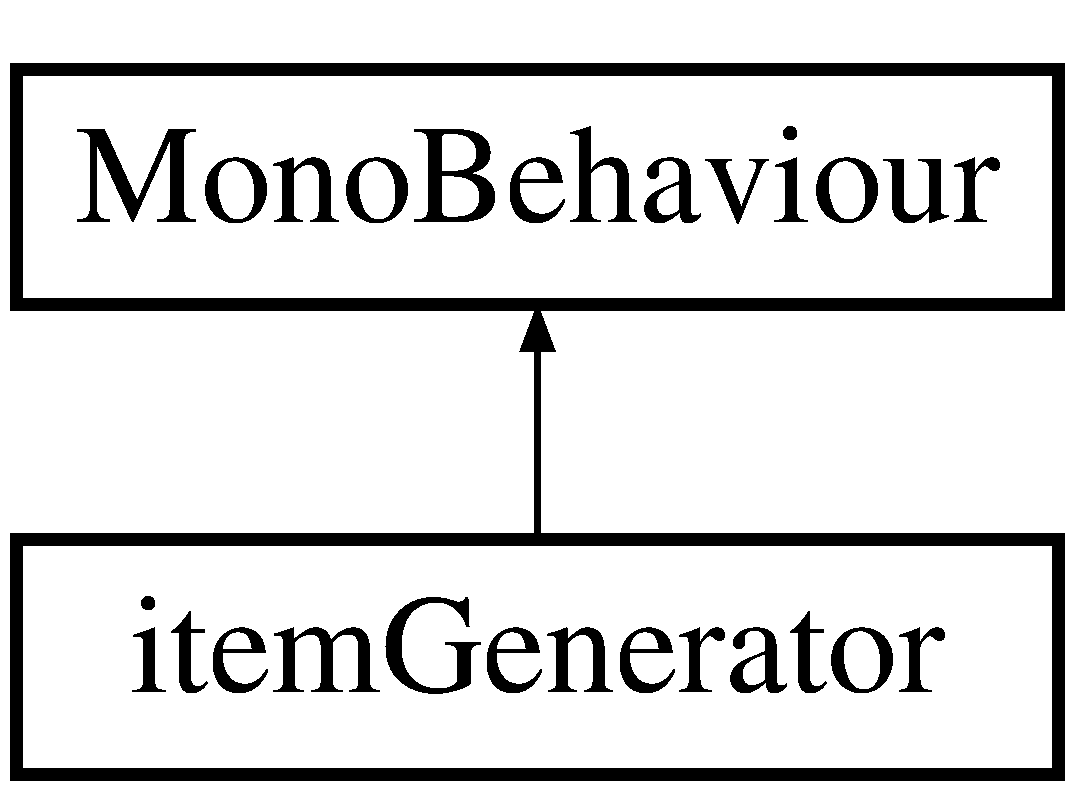
\includegraphics[height=2.000000cm]{classitem_generator}
\end{center}
\end{figure}
\subsection*{Public Member Functions}
\begin{DoxyCompactItemize}
\item 
void {\bfseries set\+Stop} ()\hypertarget{classitem_generator_a3887a75f36ad1a63fa0b06b790260379}{}\label{classitem_generator_a3887a75f36ad1a63fa0b06b790260379}

\item 
void {\bfseries set\+Start} ()\hypertarget{classitem_generator_ac60c74b86f9e461cb80c705ce38d94d2}{}\label{classitem_generator_ac60c74b86f9e461cb80c705ce38d94d2}

\end{DoxyCompactItemize}
\subsection*{Static Public Member Functions}
\begin{DoxyCompactItemize}
\item 
static Game\+Object\mbox{[}$\,$\mbox{]} {\bfseries Find\+Game\+Objects\+With\+Tag} (string tag)\hypertarget{classitem_generator_a4d3ffcf511724da55ee037738938a3e9}{}\label{classitem_generator_a4d3ffcf511724da55ee037738938a3e9}

\end{DoxyCompactItemize}
\subsection*{Public Attributes}
\begin{DoxyCompactItemize}
\item 
Game\+Object {\bfseries tornado\+Center}\hypertarget{classitem_generator_a7a3c094dee2b917d489a462cc369561b}{}\label{classitem_generator_a7a3c094dee2b917d489a462cc369561b}

\item 
Game\+Object {\bfseries diamond}\hypertarget{classitem_generator_a9f986797e5ee5769207ddd26bda3cb6c}{}\label{classitem_generator_a9f986797e5ee5769207ddd26bda3cb6c}

\item 
Game\+Object {\bfseries bomb}\hypertarget{classitem_generator_a2b3fb9d879b486ba187d0782d6224b6e}{}\label{classitem_generator_a2b3fb9d879b486ba187d0782d6224b6e}

\item 
Game\+Object {\bfseries bomb\+Eff}\hypertarget{classitem_generator_aaef3d099074fb65ee61af63f142b681a}{}\label{classitem_generator_aaef3d099074fb65ee61af63f142b681a}

\item 
int {\bfseries item\+State}\hypertarget{classitem_generator_a555ee98b3fe7bb9fb5f4b792a2e565d1}{}\label{classitem_generator_a555ee98b3fe7bb9fb5f4b792a2e565d1}

\item 
int {\bfseries last\+Item\+State}\hypertarget{classitem_generator_a7440dfca610aa0d703f9dd0cd1cd100b}{}\label{classitem_generator_a7440dfca610aa0d703f9dd0cd1cd100b}

\item 
bool {\bfseries can\+Gen}\hypertarget{classitem_generator_a9a661debb6aee81ce1113303186a89c2}{}\label{classitem_generator_a9a661debb6aee81ce1113303186a89c2}

\item 
Transform {\bfseries boundary\+Min}\hypertarget{classitem_generator_af6dadcb6f3ee6e9d5574bfa9d617e3e3}{}\label{classitem_generator_af6dadcb6f3ee6e9d5574bfa9d617e3e3}

\item 
Transform {\bfseries boundary\+Max}\hypertarget{classitem_generator_ad96cb8762c2211a57a6e7b8efbba842d}{}\label{classitem_generator_ad96cb8762c2211a57a6e7b8efbba842d}

\item 
int {\bfseries cur\+Time}\hypertarget{classitem_generator_a99af826d033d9f04dc4c5cdd788fe964}{}\label{classitem_generator_a99af826d033d9f04dc4c5cdd788fe964}

\end{DoxyCompactItemize}


The documentation for this class was generated from the following file\+:\begin{DoxyCompactItemize}
\item 
Assets/\+Scripts/item\+Generator.\+cs\end{DoxyCompactItemize}

\hypertarget{classmenu}{}\section{menu Class Reference}
\label{classmenu}\index{menu@{menu}}
Inheritance diagram for menu\+:\begin{figure}[H]
\begin{center}
\leavevmode
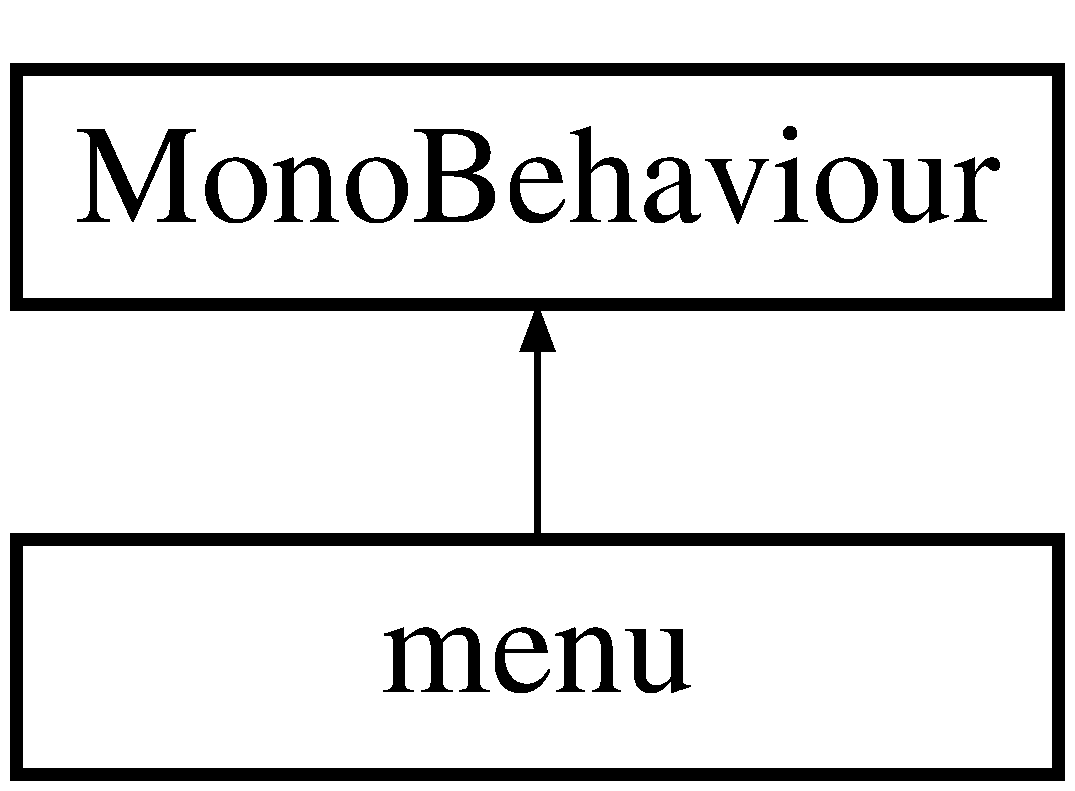
\includegraphics[height=2.000000cm]{classmenu}
\end{center}
\end{figure}
\subsection*{Public Member Functions}
\begin{DoxyCompactItemize}
\item 
void {\bfseries Exit\+Press} ()\hypertarget{classmenu_a2dd506a78a3b85b52f7e89d2e22ff0e4}{}\label{classmenu_a2dd506a78a3b85b52f7e89d2e22ff0e4}

\item 
void {\bfseries No\+Press} ()\hypertarget{classmenu_a92d752ec5a88de7c2beef0ef27df6c26}{}\label{classmenu_a92d752ec5a88de7c2beef0ef27df6c26}

\item 
void {\bfseries Start\+Level} ()\hypertarget{classmenu_a824aa861449f137ab3b8dc8d63d44ab2}{}\label{classmenu_a824aa861449f137ab3b8dc8d63d44ab2}

\item 
void {\bfseries Exit\+Game} ()\hypertarget{classmenu_ac054ced4ef2cae218a1d6b64ee1600a2}{}\label{classmenu_ac054ced4ef2cae218a1d6b64ee1600a2}

\end{DoxyCompactItemize}
\subsection*{Public Attributes}
\begin{DoxyCompactItemize}
\item 
Canvas {\bfseries quit\+Menu}\hypertarget{classmenu_a225342d46067d7b47f96f33b8fdb5216}{}\label{classmenu_a225342d46067d7b47f96f33b8fdb5216}

\item 
Button {\bfseries start\+Text}\hypertarget{classmenu_afd045bf4b6b334380f29f985c59da14f}{}\label{classmenu_afd045bf4b6b334380f29f985c59da14f}

\item 
Button {\bfseries exit\+Text}\hypertarget{classmenu_a07b6ccc44f63d87911b2b2170479ea7a}{}\label{classmenu_a07b6ccc44f63d87911b2b2170479ea7a}

\end{DoxyCompactItemize}


The documentation for this class was generated from the following file\+:\begin{DoxyCompactItemize}
\item 
Assets/\+Scripts/menu.\+cs\end{DoxyCompactItemize}

\hypertarget{class_player_health}{}\section{Player\+Health Class Reference}
\label{class_player_health}\index{Player\+Health@{Player\+Health}}
Inheritance diagram for Player\+Health\+:\begin{figure}[H]
\begin{center}
\leavevmode
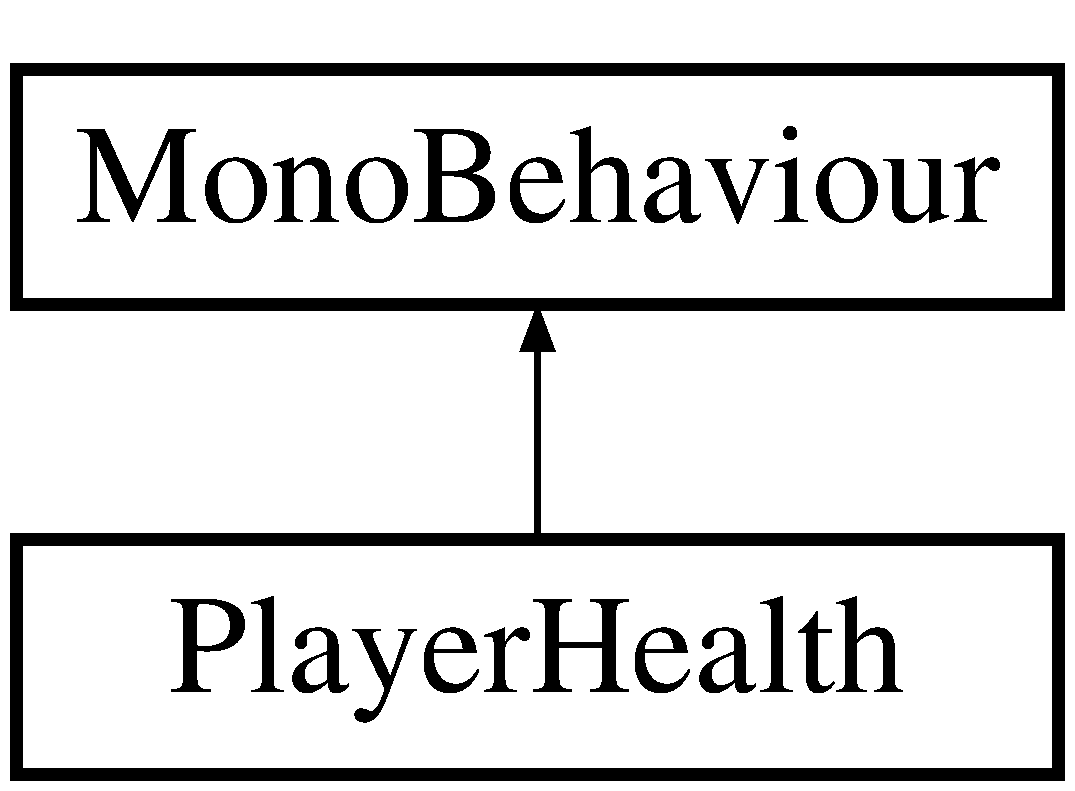
\includegraphics[height=2.000000cm]{class_player_health}
\end{center}
\end{figure}
\subsection*{Public Member Functions}
\begin{DoxyCompactItemize}
\item 
void {\bfseries decrease\+Health} (float dmg)\hypertarget{class_player_health_aa496009bbd761011fdac86f070deaa18}{}\label{class_player_health_aa496009bbd761011fdac86f070deaa18}

\item 
void {\bfseries Set\+Health\+Bar} (float my\+Health)\hypertarget{class_player_health_a3846c3773f237618f3a5bbbe1e1ae203}{}\label{class_player_health_a3846c3773f237618f3a5bbbe1e1ae203}

\end{DoxyCompactItemize}
\subsection*{Public Attributes}
\begin{DoxyCompactItemize}
\item 
float {\bfseries max\+\_\+\+Health}\hypertarget{class_player_health_a5bd2cfbe75c653125f0d50db46a18be0}{}\label{class_player_health_a5bd2cfbe75c653125f0d50db46a18be0}

\item 
Game\+Object {\bfseries health\+Bar}\hypertarget{class_player_health_a9e05e6010af085577184984d05578eb8}{}\label{class_player_health_a9e05e6010af085577184984d05578eb8}

\end{DoxyCompactItemize}


The documentation for this class was generated from the following file\+:\begin{DoxyCompactItemize}
\item 
Assets/\+Scripts/Player\+Health.\+cs\end{DoxyCompactItemize}

\hypertarget{classsound}{}\section{sound Class Reference}
\label{classsound}\index{sound@{sound}}
Inheritance diagram for sound\+:\begin{figure}[H]
\begin{center}
\leavevmode
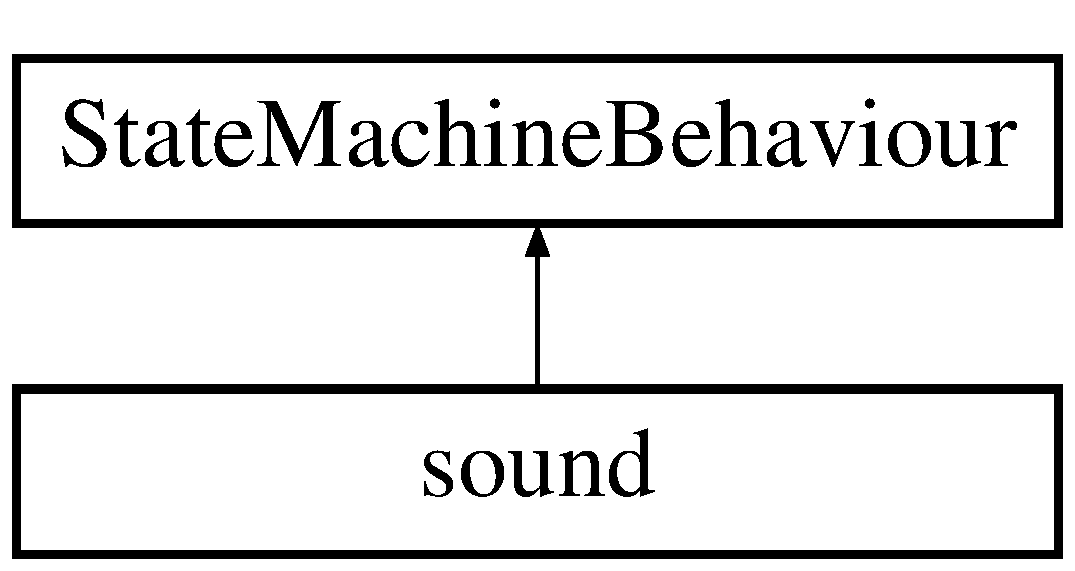
\includegraphics[height=2.000000cm]{classsound}
\end{center}
\end{figure}
\subsection*{Public Member Functions}
\begin{DoxyCompactItemize}
\item 
override void {\bfseries On\+State\+Enter} (Animator animator, Animator\+State\+Info state\+Info, int layer\+Index)\hypertarget{classsound_a2e6970c535fadf7c146a8a5b06aca4ea}{}\label{classsound_a2e6970c535fadf7c146a8a5b06aca4ea}

\item 
override void {\bfseries On\+State\+Update} (Animator animator, Animator\+State\+Info state\+Info, int layer\+Index)\hypertarget{classsound_acb1dd2017bcf36ff10c66bddc49074c8}{}\label{classsound_acb1dd2017bcf36ff10c66bddc49074c8}

\end{DoxyCompactItemize}
\subsection*{Public Attributes}
\begin{DoxyCompactItemize}
\item 
Audio\+Clip {\bfseries sound\+Effect}\hypertarget{classsound_a240d4bcb27d12691404853bd07eda1e9}{}\label{classsound_a240d4bcb27d12691404853bd07eda1e9}

\end{DoxyCompactItemize}
\subsection*{Protected Attributes}
\begin{DoxyCompactItemize}
\item 
P\+Qchan\+Controller {\bfseries chan}\hypertarget{classsound_ae5d531a863726cffc00ad4cf26a1fa30}{}\label{classsound_ae5d531a863726cffc00ad4cf26a1fa30}

\end{DoxyCompactItemize}


The documentation for this class was generated from the following file\+:\begin{DoxyCompactItemize}
\item 
Assets/\+Scripts/sound.\+cs\end{DoxyCompactItemize}

\hypertarget{classtornado_movement}{}\section{tornado\+Movement Class Reference}
\label{classtornado_movement}\index{tornado\+Movement@{tornado\+Movement}}
Inheritance diagram for tornado\+Movement\+:\begin{figure}[H]
\begin{center}
\leavevmode
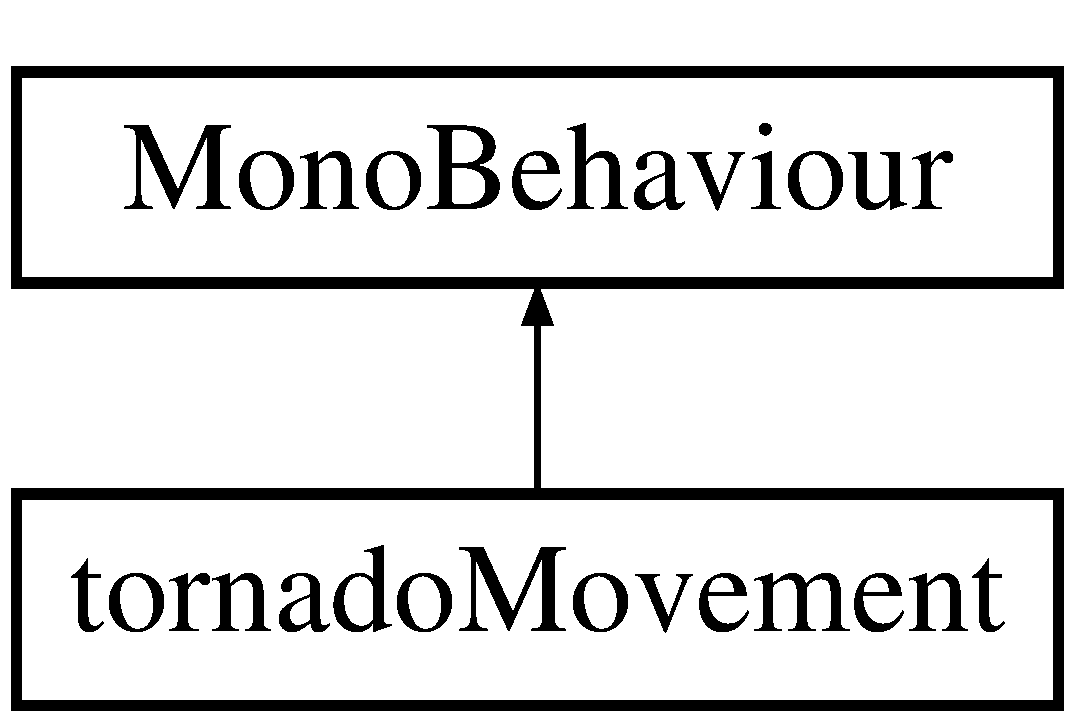
\includegraphics[height=2.000000cm]{classtornado_movement}
\end{center}
\end{figure}
\subsection*{Public Member Functions}
\begin{DoxyCompactItemize}
\item 
void {\bfseries set\+Move} ()\hypertarget{classtornado_movement_a3b1a15b4bda9073c07447c61be5cc461}{}\label{classtornado_movement_a3b1a15b4bda9073c07447c61be5cc461}

\item 
void {\bfseries set\+Stop} ()\hypertarget{classtornado_movement_a0b376571a680bb4f4472f18701d7bfbf}{}\label{classtornado_movement_a0b376571a680bb4f4472f18701d7bfbf}

\end{DoxyCompactItemize}
\subsection*{Public Attributes}
\begin{DoxyCompactItemize}
\item 
Game\+Object {\bfseries tornado}\hypertarget{classtornado_movement_aeaadb73cee71f880f17537dfac0f5972}{}\label{classtornado_movement_aeaadb73cee71f880f17537dfac0f5972}

\item 
bool {\bfseries can\+Move}\hypertarget{classtornado_movement_ae3a24d1980d9d27b88e74cab7dc873a6}{}\label{classtornado_movement_ae3a24d1980d9d27b88e74cab7dc873a6}

\end{DoxyCompactItemize}


The documentation for this class was generated from the following file\+:\begin{DoxyCompactItemize}
\item 
Assets/\+Scripts/tornado\+Movement.\+cs\end{DoxyCompactItemize}

%--- End generated contents ---

% Index
\backmatter
\newpage
\phantomsection
\clearemptydoublepage
\addcontentsline{toc}{chapter}{Index}
\printindex

\end{document}
